\header{7}
\chapter{Schiemannen}
\section{Inleiding}
In dit hoofdstuk worden de knopen geleerd die belangrijk zijn tijdens het varen. Je moet de knopen kunnen maken en begrijpen wanneer en waarom je ze gebruikt. Ook word je geacht een aantal verschillende soorten touwen te kunnen onderscheiden en hun voordelen te begrijpen.

\section{Touwsoorten, toepassing en terminologie}

\paragraph{Gevlochten en geslagen}
Een touw kan opgebouwd worden op twee manieren: geslagen en gevlochten. Beide touwen hebben voor- en nadelen waardoor er niet één superieur is aan de ander. Waar een geslagen touw vaak goedkoper is, loopt een gevlochten touw soepeler door blokken. Om deze redenen zie je vaak beide touwen op een boot.

\paragraph{Schavielen}
Wanneer een touw constant op dezelfde plek ergens tegen aan schuurt, is deze aan het schavielen. Dit kan bijvoorbeeld gebeuren wanneer je afgemeerd bent en een landvast tegen de kade schuurt. Een dweil tussen je landvast en de kade kan dit verhelpen.

\paragraph{Touwsoorten}
Tegenwoordig wordt aan boord voornamelijk touw van kunstvezel gebruikt waar dit vroeger veel natuurvezeltouw was. Om de sterktes en zwaktes van een kunstvezel touw beter te begrijpen is in tabel \ref{table:touwwerk} een vergelijking gemaakt tussen de twee touwsoorten.

\begin{table}[h]
	\centering
	\caption{Verschil in touwsoorten}
	\label{table:touwwerk}
	\begin{tabular}{c|c}
		\textbf{Natuurvezel} & \textbf{Kunstvezel} \\ \hline
		Rek en krimpen bij nat en droog worden & Geen rek \\ \hline
		Geringe breeksterkte & Hoge breeksterkte \\ \hline
		Bestand tegen UV-straling & Matig bestand tegen UV-straling \\ \hline
		Slijtvast bij schavielen & Gevoelig voor schavielen
	\end{tabular}
\end{table}

\paragraph{Toepassingen soorten touw}
Verschillende situaties vragen om verschillende touwsoorten. Hieronder is een kort overzicht van het meest geschikte touw voor verschillende situaties.
\begin{itemize}
	\item \textbf{Schoten:} Schoten moeten soepel door de blokken lopen voor gebruiksgemak. Dit maakt een gevlochten touw erg geschikt.
	\item \textbf{Ankerlijn en landvasten:} Voor landvasten en ankerlijnen is een kleine mate van rek gunstig. Deze vangen namelijk de klappen van plotselinge bewegingen op.
	\item \textbf{Vallen:} Voor een val is een touw zonder rek belangrijk. Dit maakt het hijsen makkelijker en voorkomt dat deze zeilen later `inzakken'.
\end{itemize}


\section{De knopen}
\subsection{Halve steek \hfill \hspace{2 cm} \textit{Figuur \ref{pic:halve_steek}} } 
Een halve steek leg je wanneer je een lijn vast wil leggen waar weinig kracht op komt. De halve steek is de basis voor veel knopen en steken.
\subsection{Slipsteek \hfill \textit{Figuur \ref{pic:slip_steek}}}
De slipsteek kan alleen gebruikt worden in situaties waar weinig kracht op de lijn komt. Het voordeel van een slipsteek is dat hij snel los te maken is.
\subsection{Achtknoop \hfill \textit{Figuur \ref{pic:achtknoop}}}
Een achtknoop wordt gebruikt om een verdikking in een lijn te maken. Hiermee voorkom je bijvoorbeeld dat een lijn door een blok schiet. 

\begin{figure}[h]
  \centering
  \begin{minipage}[b]{0.32\textwidth}
  \centering
    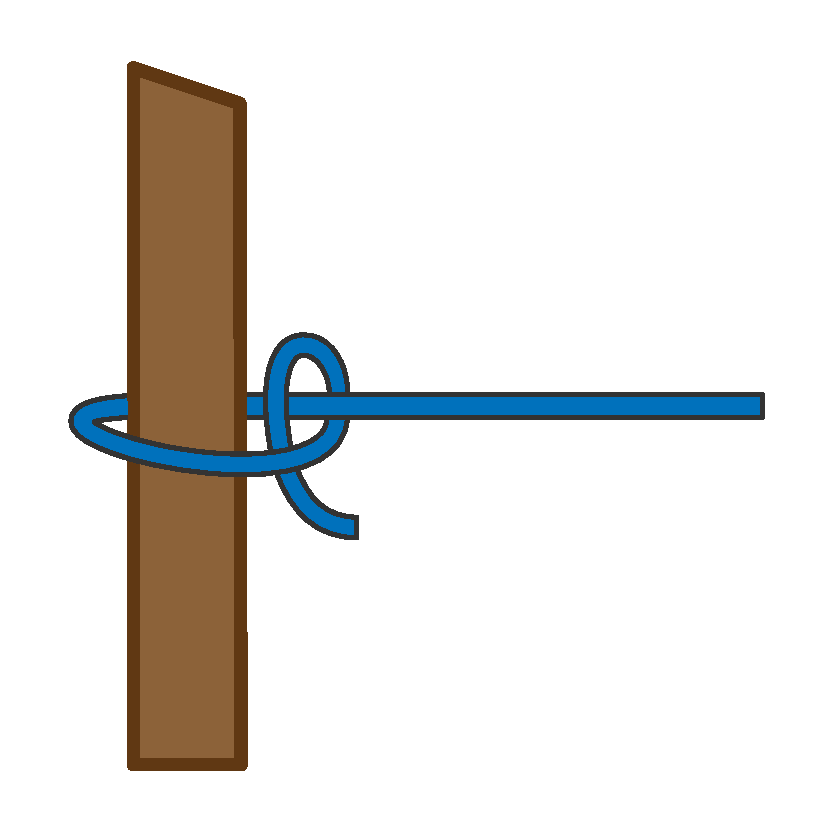
\includegraphics[height=4cm]{Hoofdstukken/Schiemannen/pdf/halve_steek.pdf}
    \caption{Halve steek}
    \label{pic:halve_steek}
  \end{minipage}
  \hfill
  \begin{minipage}[b]{0.32\textwidth}
    \centering
    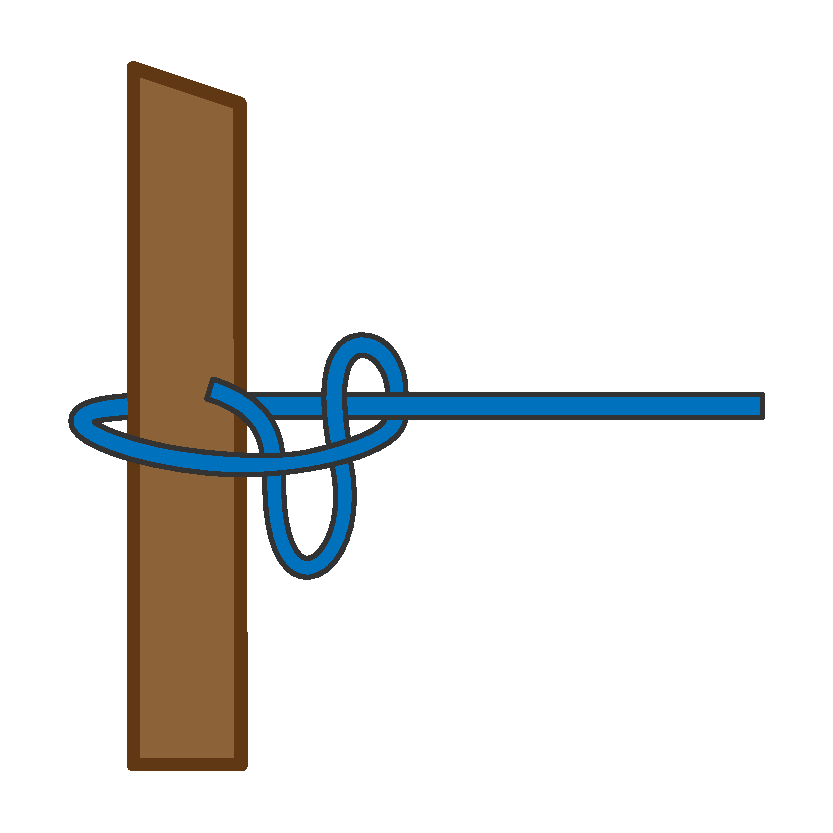
\includegraphics[height=4cm]{Hoofdstukken/Schiemannen/pdf/slip_steek.pdf}
    \caption{Slipsteek}
    \label{pic:slip_steek}
    \end{minipage}
  \hfill
  \begin{minipage}[b]{0.32\textwidth}
    \centering
    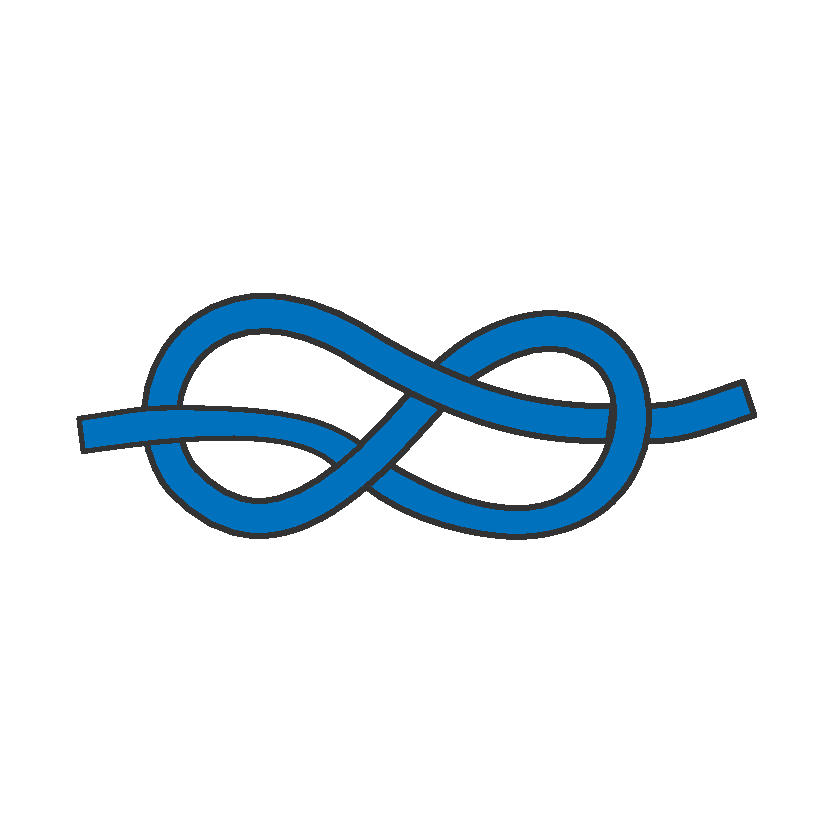
\includegraphics[height=4cm]{Hoofdstukken/Schiemannen/pdf/achtknoop.pdf}
    \caption{Achtknoop}
    \label{pic:achtknoop}
  \end{minipage}
\end{figure}

\subsection{Platte knoop \hfill \textit{Figuur \ref{pic:platte_knoop}}}
Deze knoop is geschikt voor het verbinden van twee uiteinde van een lijn van gelijke dikte. Deze knoop is niet geschikt voor situaties waar veel kracht op de lijn komt te staan. Hiervoor is een schootsteek beter geschikt.
\subsection{Schootsteek \hfill \textit{Figuur \ref{pic:schoot_steek}}}
Een schootsteek is geschikt om twee lijnen van ongelijke dikte aan elkaar te maken. De knoop is ook geschikt voor lijnen van gelijke dikte en kan veel kracht aan. Bij lijnen van ongelijke dikte wordt met de dikke lijn de `lus' (blauw) gelegd, dit maakt de knoop makkelijker. Wanneer er extreem veel kracht op de knoop komt, kan deze dubbel gelegd worden. In dit geval wordt de `lus' een extra keer omwikkeld. 
 
\begin{figure}[h]
  \centering
  \begin{minipage}[b]{0.32\textwidth}
  \centering
    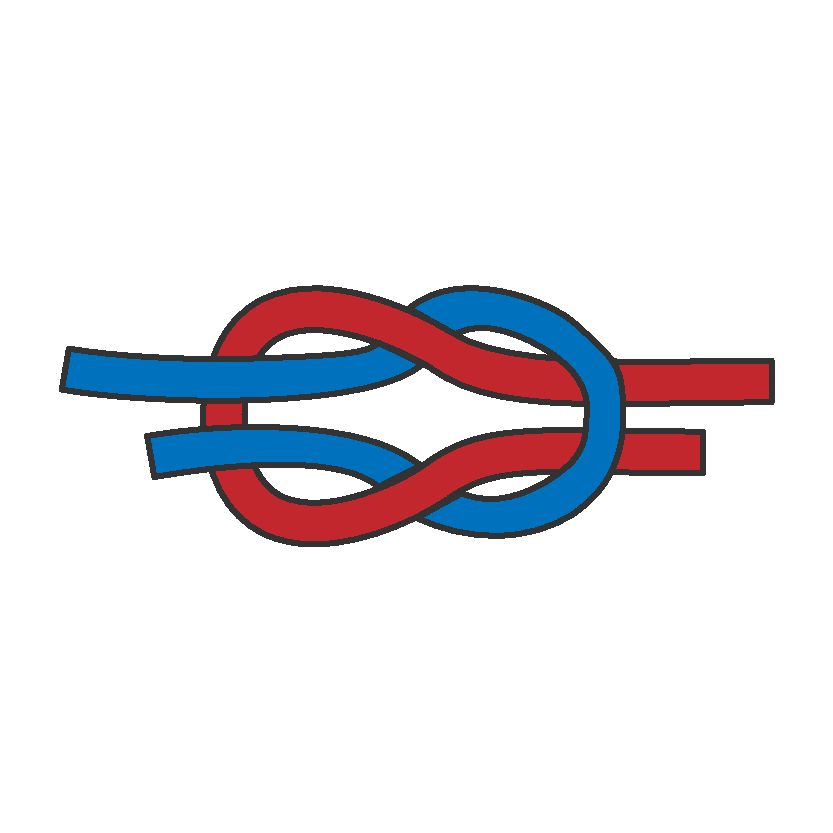
\includegraphics[height=4cm]{Hoofdstukken/Schiemannen/pdf/platteknoop.pdf}
    \caption{Platte knoop}
    \label{pic:platte_knoop}
  \end{minipage}
  \hfill
  \begin{minipage}[b]{0.64\textwidth}
    \centering
    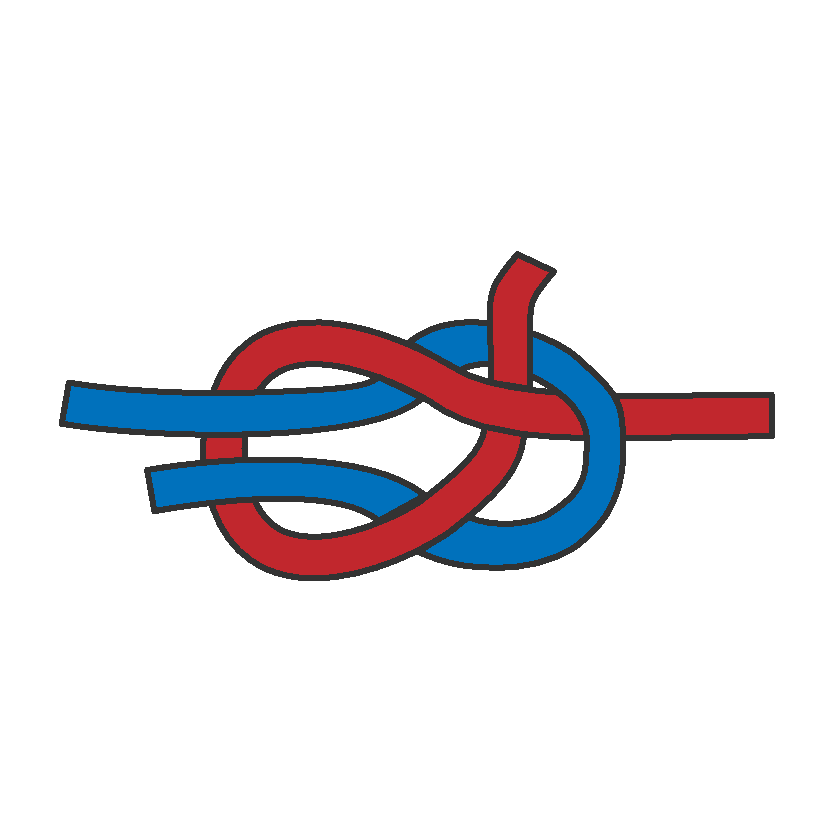
\includegraphics[height=4cm]{Hoofdstukken/Schiemannen/pdf/schootsteek.pdf}
    \hspace*{1cm}
    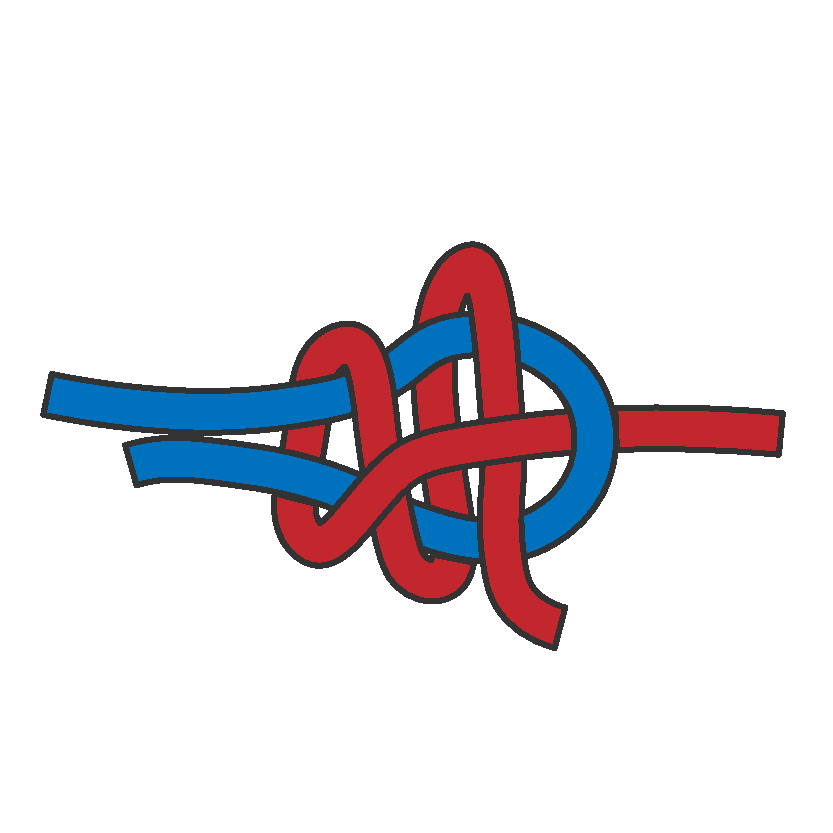
\includegraphics[height=4cm]{Hoofdstukken/Schiemannen/pdf/dubbele_schootsteek.pdf}
    \caption{Schootsteek enkel en dubbel}
    \label{pic:schoot_steek}
    \end{minipage}
  \hfill
\end{figure}
\subsection{Mastworp \hfill \textit{Figuur \ref{pic:mastworp}}}
Deze knoop wordt veel gebruikt in pionieren en om je boot aan te leggen. De knoop trekt zich zelf strakker naar mate er meer kracht op komt. Daarnaast kun je een slipsteek op een mastworp leggen. Dit voorkomt dat de mastworp los kan schieten als er veel aan getrokken wordt.
\subsection{Paalsteek \hfill \textit{Figuur \ref{pic:paal_steek}}} 
De paalsteek is bedoeld om een niet slippende lus in een lijn te leggen. De lus is erg sterk, maar kan wel gemakkelijk weer losgehaald worden.
\subsection{Een tros opschieten \hfill \textit{Figuur \ref{pic:opschieten}}}
Een tros opschieten is een manier om een lijn op te bergen zonder dat deze in de knoop raakt. Tijdens het opschieten maak je een aantal gelijke lussen. Aan het einde wikkel je de rest van de lijn om de lussen en leg je een knoop als in het figuur. Opschieten staat ook wel bekend als opbossen.
\begin{figure}[h]
  \centering
  \begin{minipage}[b]{0.32\textwidth}
  \centering
    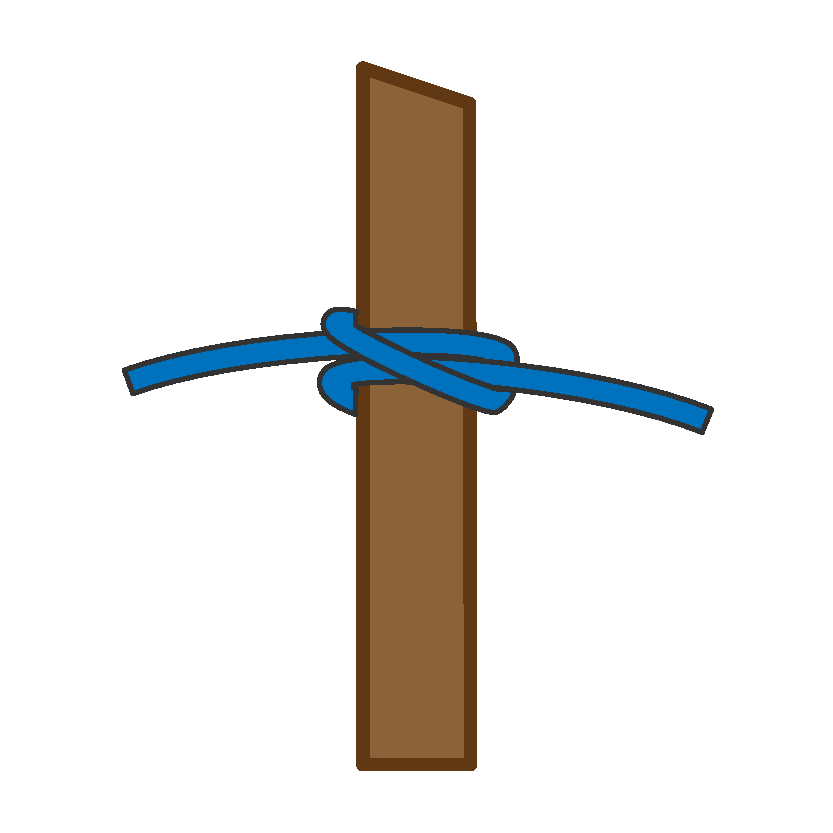
\includegraphics[height=4cm]{Hoofdstukken/Schiemannen/pdf/mastworp.pdf}
    \caption{Mastworp}
    \label{pic:mastworp}
  \end{minipage}
  \hfill
  \begin{minipage}[b]{0.32\textwidth}
    \centering
    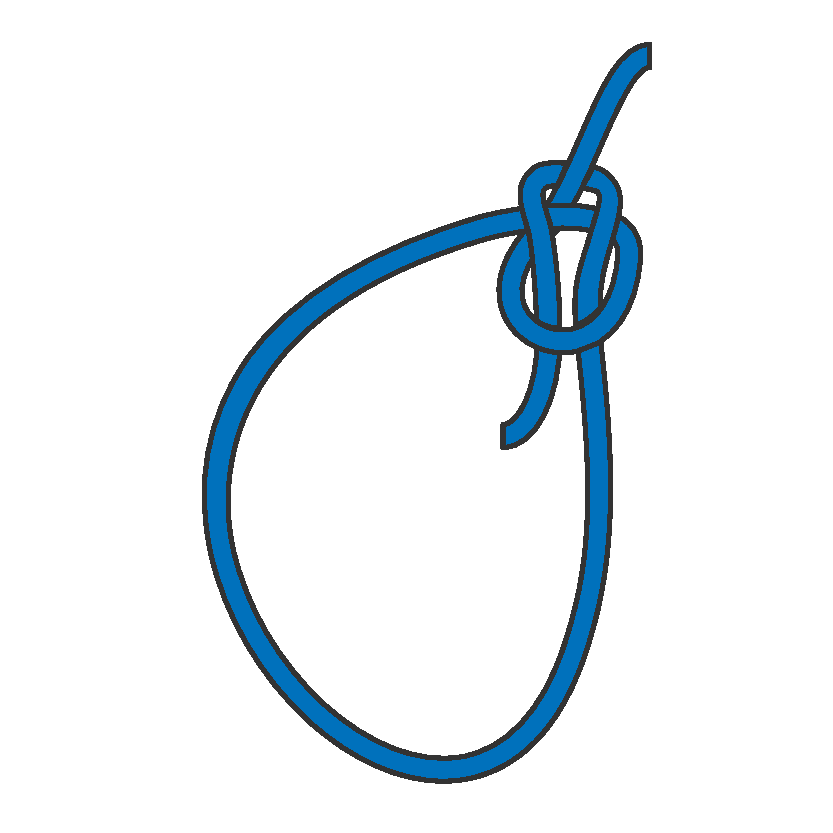
\includegraphics[height=4cm]{Hoofdstukken/Schiemannen/pdf/paalsteek.pdf}
    \caption{Paalsteek}
    \label{pic:paal_steek}
    \end{minipage}
  \hfill
   \begin{minipage}[b]{0.32\textwidth}
    \centering
    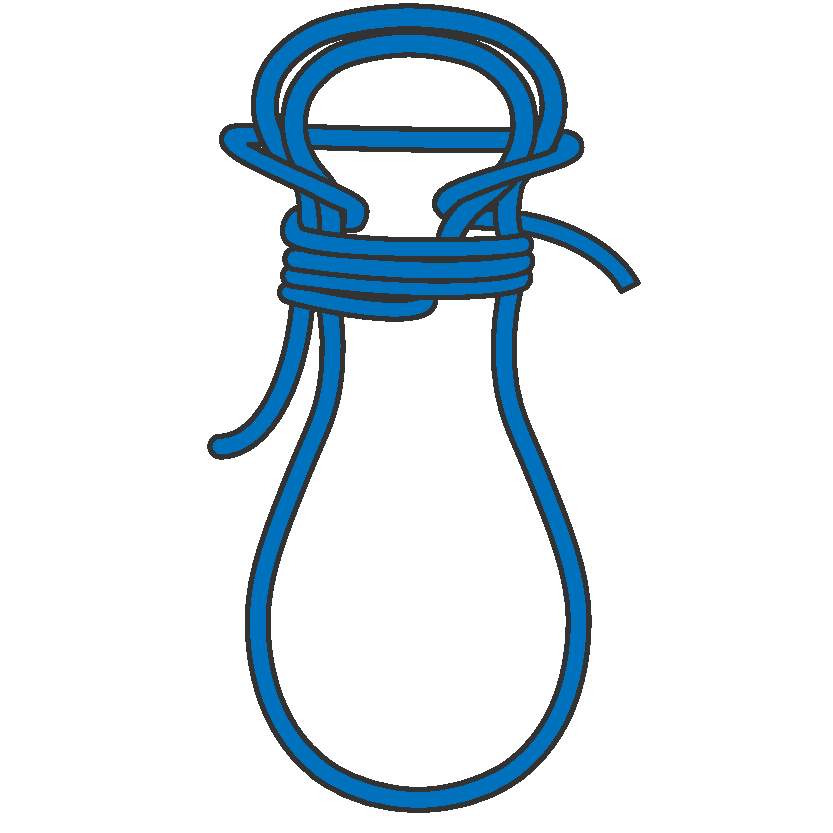
\includegraphics[height=4cm]{Hoofdstukken/Schiemannen/pdf/opbossen.pdf}
    \caption{Opschieten}
    \label{pic:opschieten}
    \end{minipage}
\end{figure}


\subsection{Dubbele halve steek \hfill \textit{Figuur \ref{pic:dub_halve_steek} \& \ref{pic:dub_slip_halve_steek}}}
Een dubbele halve steek is geschikt om lijnen strak aan een oog vast te maken. Dit is bijvoorbeeld handig als aan wilt leggen met een meerpen. Je wikkelt eerst de lijn tweemaal om een oog en legt er vervolgens twee halve steken in. Dit maakt een mastworp. Je kan de eerste halve steek ook vervangen door een slipsteek om hem makkelijker los te maken. Dit is te zien in figuur \ref{pic:dub_slip_halve_steek}.


\begin{figure}[h]
	\centering
	\begin{minipage}[b]{0.49\textwidth}
		\centering
		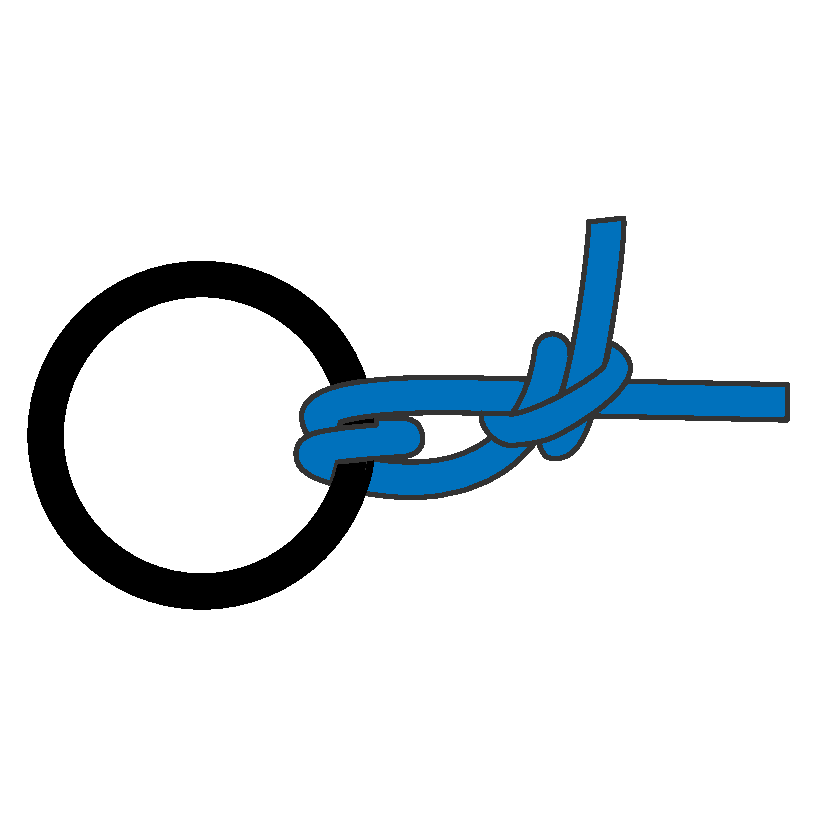
\includegraphics[height=4cm]{Hoofdstukken/Schiemannen/pdf/dubble_halve_steek.pdf}
		\caption{Dubbele halve steek}
		\label{pic:dub_halve_steek}
	\end{minipage}
	\hfill
	\begin{minipage}[b]{0.49\textwidth}
		\centering
		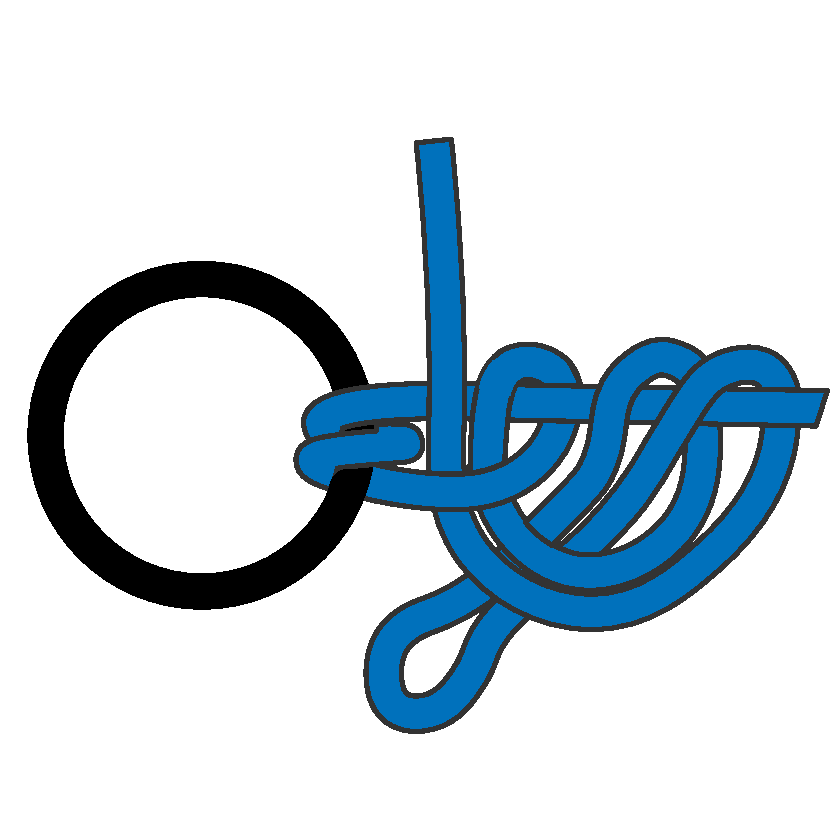
\includegraphics[height=4cm]{Hoofdstukken/Schiemannen/pdf/dubble_halve_steek_slippend.pdf}
		\caption{Slippende dubbele halve steek}
		\label{pic:dub_slip_halve_steek}
	\end{minipage}
	\hfill
\end{figure}
\newpage
\subsection{Een kikker beleggen \hfill \textit{Figuur \ref{pic:kikker1}, \ref{pic:kikker2} \& \ref{pic:kikker3}}}
Wanneer je een kikker belegt, leg je een lijn vast op een kikker. Dit is nodig voor bijvoorbeeld het hijsen van het zeil. Belangrijk bij het beleggen van een kikker in een boot is dat je de ''eindlus'' aan de bovenzijde van de kikker legt. Anders kan deze er afvallen en de kikker losraken. Daarnaast moet je het lusje zo draaien dat het uiteinde weer in de richting van het vorige achtje gaat.
\begin{figure}[h]
  \centering
  \begin{minipage}[b]{0.32\textwidth}
  \centering
    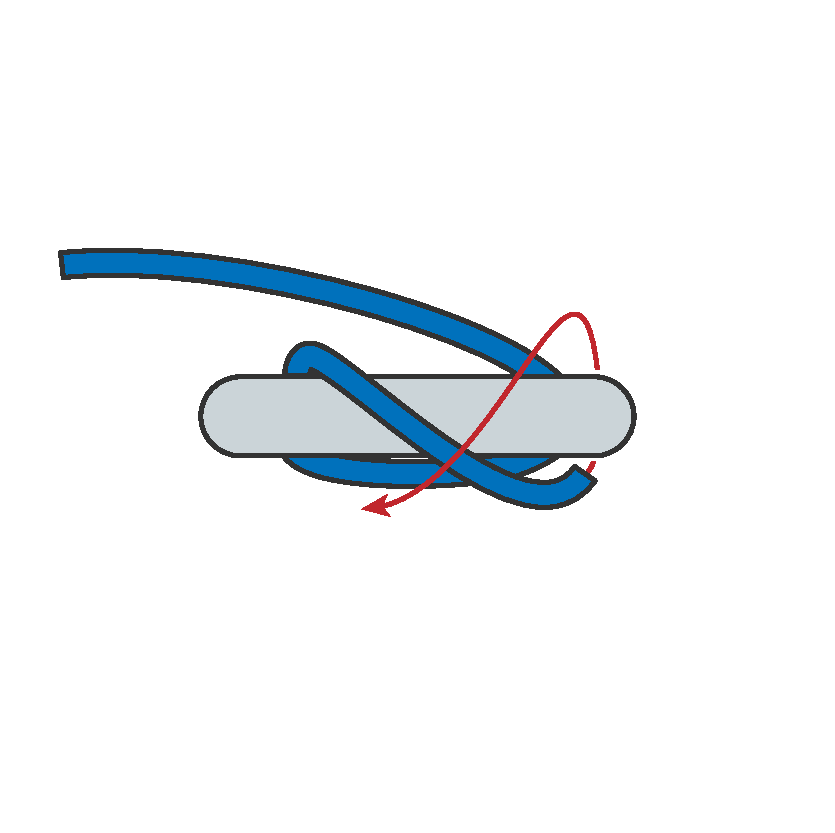
\includegraphics[width=\textwidth]{Hoofdstukken/Schiemannen/pdf/kikker1.pdf}
    \caption{Kikker 8'tjes}
    \label{pic:kikker1}
  \end{minipage}
  \hfill
  \begin{minipage}[b]{0.32\textwidth}
    \centering
    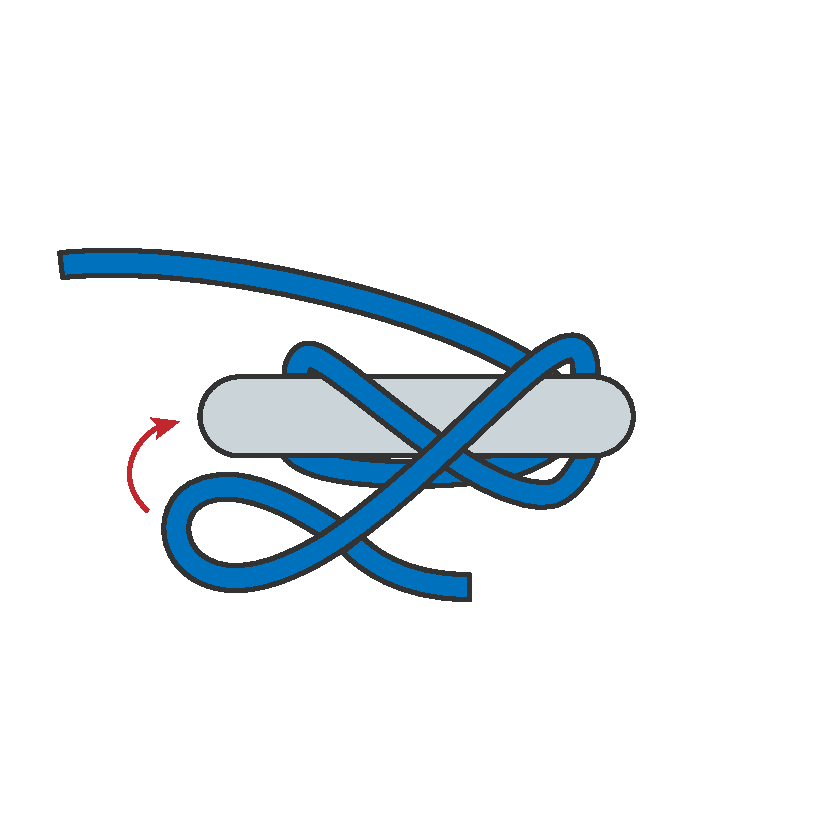
\includegraphics[width=\textwidth]{Hoofdstukken/Schiemannen/pdf/kikker2.pdf}
    \caption{Kikker eind lus}
    \label{pic:kikker2}
    \end{minipage}
  \hfill
   \begin{minipage}[b]{0.32\textwidth}
    \centering
    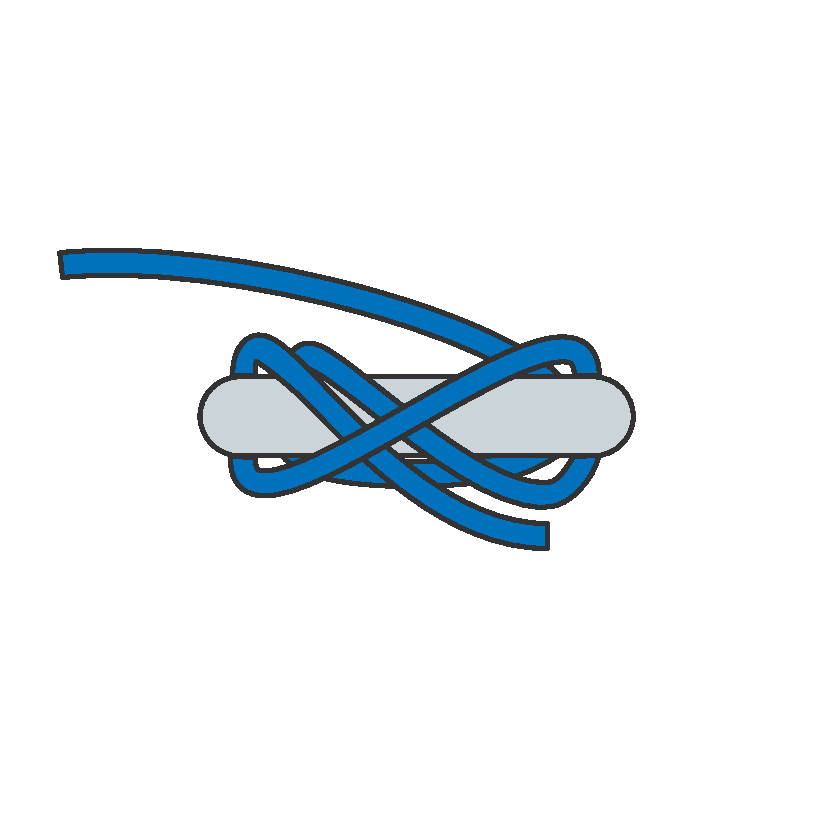
\includegraphics[width=\textwidth]{Hoofdstukken/Schiemannen/pdf/kikker3.pdf}
    \caption{Kikker afknopen}
    \label{pic:kikker3}
    \end{minipage}
\end{figure}
\section{Conclusie}
Na het lezen van dit hoofdstuk en het oefenen met de knopen, snap je het nut en toepassing van de verschillende knopen. Ook kan je alle knopen zonder voorbeeld leggen. Een instructeur heeft dit in de onderstaande tabel afgetekend.
\vspace{2cm}
\begin{table}[H]
\centering
\caption{Aftekenen knopen}
\label{my-label}
\begin{tabular}{|l|l|l|}
\hline
\textbf{Knoop of Handeling}  & \textbf{Paraaf} & \textbf{Paraaf} \\ \hline
\textit{Halve Steek}         &                 &                 \\ \hline
\textit{Slipsteek}          &                 &                 \\ \hline
\textit{Achtknoop}           &                 &                 \\ \hline
\textit{Platte Knoop}        &                 &                 \\ \hline
\textit{Schootsteek}        &                 &                 \\ \hline
\textit{Dubbele schootsteek}        &                 &                 \\ \hline
\textit{Mastworp}            &                 &                 \\ \hline
\textit{Paalsteek}           &                 &                 \\ \hline
\textit{Dubbele halve steek} &                 &                 \\ \hline
\textit{Slippende dubbele halve steek} &                 &                 \\ \hline
\textit{Tros opschieten}     &                 &                 \\ \hline
\textit{Kikker beleggen}     &                 &                 \\ \hline
\end{tabular}
\end{table}